\documentclass[a4paper,12pt]{article}
%%%%%%%%%%%%%%%%%%%%%%%%%%%%%%%%%%%%%%%%%%%%%%%%%%%%%%%%%%%%%%%%%%%%%%%%%%%%%%%%%%%%%%%%%%%%%%%%%%%%%%%%%%%%%%%%%%%%%%%%%%%%%%%%%%%%%%%%%%%%%%%%%%%%%%%%%%%%%%%%%%%%%%%%%%%%%%%%%%%%%%%%%%%%%%%%%%%%%%%%%%%%%%%%%%%%%%%%%%%%%%%%%%%%%%%%%%%%%%%%%%%%%%%%%%%%
\usepackage{eurosym}
\usepackage{vmargin}
\usepackage{amsmath}
\usepackage{graphics}
\usepackage{epsfig}
\usepackage{framed}
\usepackage{subfigure}
\usepackage{fancyhdr}

\setcounter{MaxMatrixCols}{10}
%TCIDATA{OutputFilter=LATEX.DLL}
%TCIDATA{Version=5.00.0.2570}
%TCIDATA{<META NAME="SaveForMode"CONTENT="1">}
%TCIDATA{LastRevised=Wednesday, February 23, 201113:24:34}
%TCIDATA{<META NAME="GraphicsSave" CONTENT="32">}
%TCIDATA{Language=American English}

\pagestyle{fancy}
\setmarginsrb{20mm}{0mm}{20mm}{25mm}{12mm}{11mm}{0mm}{11mm}
\lhead{MA4128} \rhead{Kevin O'Brien} \chead{Multinomial Logistic Regression} %\input{tcilatex}

%http://www.electronics.dit.ie/staff/ysemenova/Opto2/CO_IntroLab.pdf
\begin{document}
%
%\tableofcontents





%http://www.strath.ac.uk/aer/materials/5furtherquantitativeresearchdesignandanalysis/unit6/multinomiallogisticregression/
\section*{Multiple Logistic Regression}
\begin{itemize}
	\item So far we have looked at the case where our dependent variable is binary, i.e. it has just two categories. However there are many nominal variables with more than two categories. 
	
	%If we look at the example we gave earlier about staying on in education post-16, you can imagine that we might want a little more detail, such as knowing whether students have stayed in mainstream education, are in vocational training, or have left education altogether. This would be a three category nominal variable.
	
	\item We therefore need methods that can model this type of dependent variable as well. Luckily we can extend the logistic regression model to do this. We call this extended method \textbf{\textit{multinomial logistic regression}}, and refer to logistic regression for dichotomous dependent variables as \textbf{\textit{binary logistic regression}}.
	
	\item The basic principle of multinomial logistic regression is similar to that for binomial logistic regression, in that it is based on the probability of membership of each category of the dependent variable.
	
	% So, in our three category example, the focus is on what the probability is of being in education, in training or not in education.
	
	\item \textbf{(Important)} The way multinomial logistic regression deals with the variables in this case is somewhat similar to the concept of dummy variables, in that it compares the probability of being in each of n-1 categories compared to a baseline or reference category. 
	\item \textbf{(Important)} In a way we can say that we are fitting n-1 separate binary logistic models, where we compare category 1 to the baseline category, then category 2 to the baseline and so on. 
	\item In practice software algorithms allow us to model the comparisons to the baseline simultaneously using maximum likelihood estimation, which is better as doing it sequentially could lead to misestimation of the standard errors. 
	\item Therefore, multinomial logistic regression is basically an extension of binary logistic regression for nominal variables with more than two categories.
\end{itemize}

%\begin{itemize}
%	\item In order to market films more effectively, movie studios want to predict what type of
%	film a moviegoer is likely to see. 
%	\item By performing a Multinomial Logistic Regression, the studio
%	can determine the strength of influence a person's age, gender, and marital/dating status has upon the type
%	of film they prefer. 
%	\item The studio can then slant the advertising campaign of a particular movie
%	toward a group of people likely to go see it. 
%\end{itemize}

%-------------------------------------------------------------------------------------%
%-https://statistics.laerd.com/spss-tutorials/multinomial-logistic-regression-using-spss-statistics.php
\newpage
\section*{Examples of Multinomial Logistic Regression}

\begin{description}
	\item[Example 1.] People's occupational choices might be influenced by their parents' occupations and their own education level. We can study the relationship of one's occupation choice with education level and parent's occupation.  The occupational choices will be the outcome variable which consists of categories of occupations.
	
	\item[Example 2.] A biologist may be interested in food choices that alligators make. Adult alligators might have difference preference than young ones. The outcome variable here will be the types of food, and the predictor variables might be the length of the alligators and other environmental variables.
	
	\item[Example 3.] Entering high school students make program choices among general program, vocational program and academic program. Their choice might be modeled using their writing score and their social economic status.
\end{description}

%-------------------------------------------------------------------------------------%

\section*{British Voting Preferences}
\begin{itemize}
	\item A researcher wanted to understand whether the political party that a person votes for can be predicted from a belief in whether tax is too high and a person's income (i.e., salary). 
	\item Therefore, the political party the participants last voted for was recorded in the politics variable and had three options: "Conservatives", "Labour" and "Liberal Democrats". When presented with the statement, "tax is too high in this country", participants had four options of how to respond: "Strongly Disagree", "Disagree", "Agree" or "Strongly Agree" and stored in the variable, \texttt{tax\_too\_high}. 
	\item The researcher also asked participants their annual income which was recorded in the income variable. As such, in variable terms, a multinomial logistic regression was run to predict politics from \texttt{tax\_too\_high} and income.
	\item 
	For the British political system, we are taking a stereotypical approach to the three major political parties, whereby the Liberal Democrats and Labour are parties in favour of high taxes and the Conservatives are a party favouring lower taxes.
	
\end{itemize}

%%%%%%%%%%%%%%%%%%%%%%%%%%%%%%%%%%%%%%%%%%%%%%%%%%%%%%%%%%%%%5

\subsection*{Implementation} 
We created three variables:
\begin{itemize} 
\item[(1)] the independent variable, \texttt{tax\_too\_high}, which has four ordered categories: "Strongly Disagree", "Disagree", "Agree" and "Strongly Agree"; 
\item[(2)] the independent variable, \texttt{income}; and 
\item[(3)] the dependent variable, politics, which has three categories: "Con", "Lab" and "Lib" (i.e., to reflect the Conservatives, Labour and Liberal Democrats).
\end{itemize}
\subsection*{Factors and Covariate}
\begin{itemize} 
\item With SPSS You need to separate the variables into covariates and factors. For these particular procedures, SPSS Statistics classifies continuous independent variables as covariates and nominal independent variables as factors. 
\item Therefore, the continuous independent variable, income, is considered a covariate. However, where you have an ordinal independent variable, such as in our example (i.e., \texttt{tax\_too\_high}), you must choose whether to consider this as a covariate or a factor. 
%In our example, it will be treated as a factor.
\item 
This table shows which of your independent variables are statistically significant. You can see that income (the "income" row) was not statistically significant because p = 0.754 (the "Sig." column). On the other hand, the \texttt{tax\_too\_high} variable (the "\texttt{tax\_too\_high}" row) was statistically significant because $p = 0.014$. There is not usually any interest in the model intercept (i.e., the "Intercept" row).
\end{itemize}
\begin{figure}[h!]
	\centering
	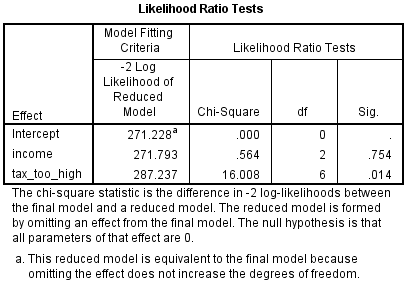
\includegraphics[width=0.7\linewidth]{images/likelihood-test}
	\caption{}
	\label{fig:likelihood-test}
\end{figure}

This table is mostly useful for nominal independent variables because it is the only table that considers the overall effect of a nominal variable, unlike the Parameter Estimates table, as shown below:


\begin{figure}[h!]
	\centering
	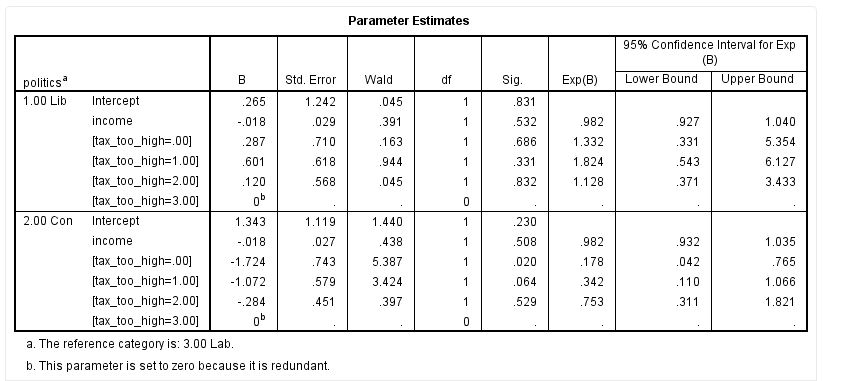
\includegraphics[width=0.7\linewidth]{multinomial}

\end{figure}
\begin{itemize}
	\item This table presents the parameter estimates (also known as the coefficients of the model). As you can see, each dummy variable has a coefficient for the \texttt{tax\_too\_high} variable. However, there is no overall statistical significance value. This was presented in the previous table (i.e., the Likelihood Ratio Tests table). 
	\item As there were three categories of the dependent variable, you can see that there are two sets of logistic regression coefficients. 
	\item The first set of coefficients are found in the "Lib" row (representing the comparison of the Liberal Democrats category to the reference category, Labour). The second set of coefficients are found in the "Con" row (this time representing the comparison of the Conservatives category to the reference category, Labour). You can see that "income" for both sets of coefficients is not statistically significant \texttt{(p = 0.532 and p = 0.508, respectively; the "Sig." column)}.
	
	\item The only coefficient (the "B" column) that is statistically significant is for the second set of coefficients. It is \texttt{[tax\_too\_high=.00] (p = 0.020)}, which is a dummy variable representing the comparison between "Strongly Disagree" and "Strongly Agree" to tax being too high. 
	\item The sign is negative, indicating that if you "strongly agree" compared to "strongly disagree" that tax is too high, you are more likely to be Conservative than Labour. However, because the coefficient does not have a simple interpretation, the exponentiated values of the coefficients (the "\texttt{Exp(B)}" column) are normally considered instead.
\end{itemize}



\section*{Summary}

Multinomial Logistic Regression is useful for situations in which you want to be able to classify
subjects based on values of a set of predictor variables. This type of regression is similar to logistic
regression, but it is more general because the dependent variable is not restricted to two categories.
\end{document}


